\hypertarget{scrapbook}{%
\subsection{Scrapbook}\label{scrapbook}}

\hypertarget{motivation}{%
\subsubsection{Motivation}\label{motivation}}

This pattern describes a way to make the project meaningful.

\hypertarget{context}{%
\subsubsection{Context}\label{context}}

We have been working together for a while now. We have maintained and
revised our pattern catalog, and we are achieving some of the ``What's
Next'' steps associated with some of the patterns.

\hypertarget{forces}{%
\subsubsection{Forces}\label{forces}}

\begin{quote}

\includegraphics{images/attention.png} \textbf{Attention}: due to
limited energy, we need to ask: where should we set the focus?

\includegraphics{images/interest.png} \textbf{Interest}: new experiences
catch our attention. 
\includegraphics{images/meaning.png}
\textbf{Meaning}: shared history makes things meaningful.
\end{quote}

\hypertarget{problem}{%
\subsubsection{Problem}\label{problem}}

Not all of the ideas we've come up with have proved workable. Not all of
the patterns we've noticed remain equally relevant. In particular, some
patterns no longer lead to concrete next steps.

\hypertarget{solution}{%
\subsubsection{Solution}\label{solution}}

In order to maintain focus, is important to ``tune'' and ``prune'' the
things we give our attention to. We can connect this understanding to
any actions undertaken in the project by asking questions like these:

\begin{quote}
(1) Review what was supposed to happen. (2) Establish what is
happening/happened. (3) Determine what's right and wrong with what we
are doing/have done. (4) What did we learn or change? (5) What else
should we change going forward? {{[}9{]}}, after {{[}10{]}}.
\end{quote}

Other review processes have been formalized, including the design review
in architecture and the postmortem in theater and other teamwork
settings {{[}7,8{]}}. The review process may benefit from having an
experienced facilitator on board {{[}6{]}}. As current priorities become
clearer, we decide where to focus. Anything that isn't receiving active
attention should be moved to a {{Scrapbook}}. This may encompass:

\begin{itemize}
\tightlist
\item
  \emph{Retired patterns} that are tabled or completed (no more next
  steps);
\item
  \emph{Proto-patterns} made of problems, issues, and concerns;
\item
  \emph{A back-catalog} of publications, reports, or other artifacts.
\end{itemize}

In the Peeragogy project, alongside our patterns we initially maintained
a collection of antipatterns (like `{{Magical thinking}}') but the next
steps coming from these seemed particularly convoluted and abstract. So,
we archived them.\footnote{\url{http://paragogy.net/Scrapbook}} problems
-- without known solutions -- right up front in the Introduction to the
\emph{Peeragogy Handbook} {{[}9{]}}. Other proto-patterns include
`{{Onboarding}}' and `{{Don't quit your day job}}', which arose in our
review of this paper (see ``Emergent Roadmap'', below). Our back-catalog
includes academic papers {{[}14{]}} and a thesis {{[}5{]}}. Everyone can
maintain their own personal {{Scrapbook}} as along with a communal one.
Furthermore, you don't need to limit yourself to \emph{your own}
creativity: include interesting ideas from other sources (see {{Reduce,
reuse, recycle}}). In some cases a designated {{Wrapper}} may have to do
further work to elicit and organize contributions.

\hypertarget{rationale}{%
\subsubsection{Rationale}\label{rationale}}

We want to keep attention focused on the most relevant issues. If a
pattern, task, or concern does not lead to concrete ``next steps'' at
the moment, sufficient time for reflection may offer a better
understanding, and it may prove useful and actionable in a different
context.

\hypertarget{resolution}{%
\subsubsection{Resolution}\label{resolution}}

Judicious use of the {{Scrapbook}} can help focus project participants'
\textbf{attention} on current concerns, without losing grasp of items of
\textbf{interest}. The currently active pattern catalog is leaner and
more action-oriented as a result. If the {{Roadmap}} shows where we're
going, it is the {{Scrapbook}} that shows most clearly where we've been,
and collects the observations that are most \textbf{meaningful} to us.

\hypertarget{example-1}{%
\subsubsection{Example 1}\label{example-1}}

The history of the Wikimedia Foundation, and of Wikipedia, are
maintained as wiki pages.\footnote{\url{https://wikimediafoundation.org/wiki/History_of_the_Wikimedia_Foundation}},\footnote{\url{https://en.wikipedia.org/wiki/Wikipedia}}
Wikipedia details outstanding issues, in the form of
critiques.\footnote{\url{https://en.wikipedia.org/wiki/Criticism_of_Wikipedia}}
available to help facilitate the process of vetting proposed
fine-grained changes to articles.\footnote{\url{https://en.wikipedia.org/wiki/Special:RecentChanges}},\footnote{\url{https://en.wikipedia.org/wiki/Wikipedia:Recent_changes_patrol\#Tools}}
typically discussed at the Village Pump, and there are mechanisms in
place for settling disputes.{[}\^{}7\^{}{]},\footnote{\url{https://en.wikipedia.org/wiki/Wikipedia:Requests_for_comment}}

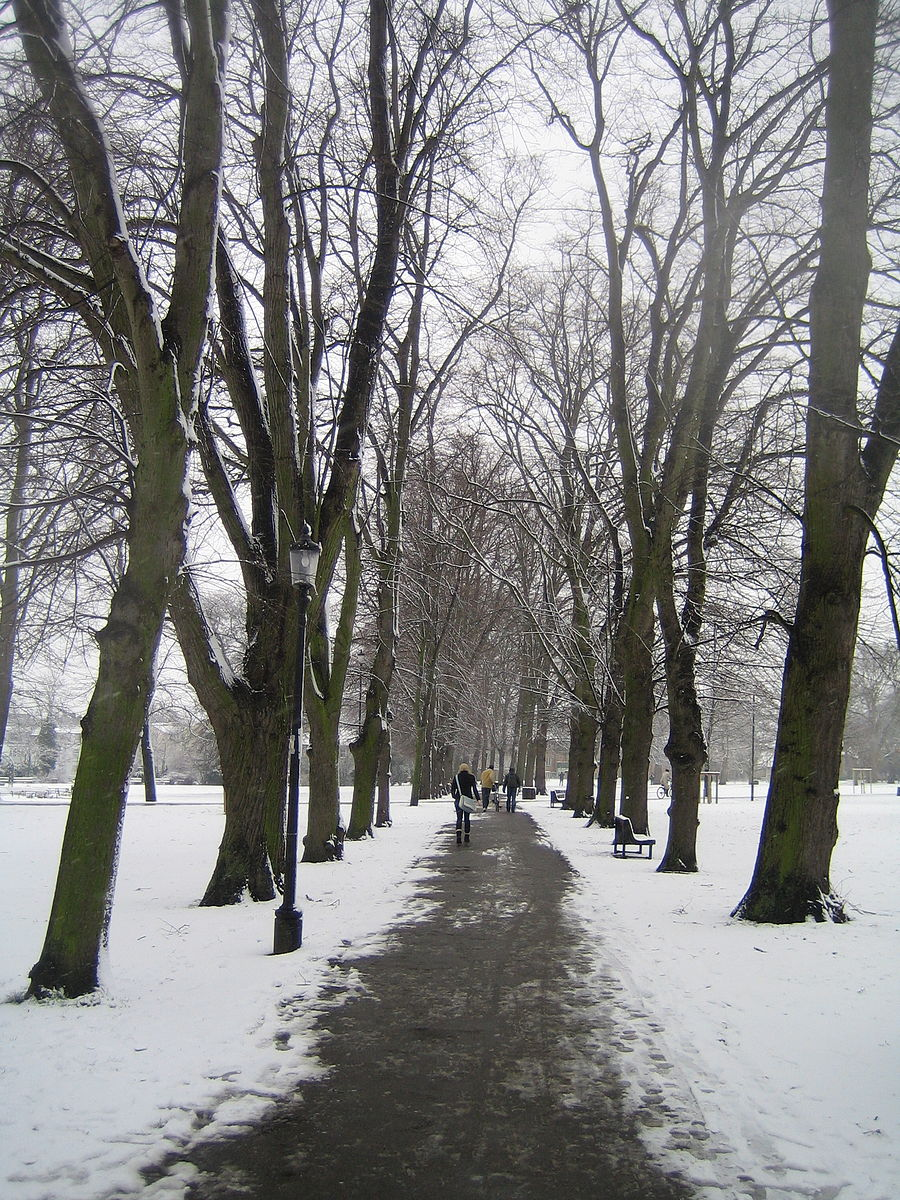
\includegraphics{images/ChristsPieces.jpg}\\
\emph{Park: Christ's Pieces, Cambridge, UK}

\hypertarget{example-2}{%
\subsubsection{Example 2}\label{example-2}}

Just as a university campus grows and changes over time, future
peeragogues will be drawn to new problems and patterns. They will trace
new paths and build new emergent structures (Figure
{[}christs-pieces{]}).

\hypertarget{whats-next-in-the-peeragogy-project}{%
\subsubsection{What's Next in the Peeragogy
Project}\label{whats-next-in-the-peeragogy-project}}

After pruning back our pattern catalog, we want it to grow again: new
patterns are needed. One strategy would be to turn the whole
\emph{Peeragogy Handbook} into design patterns.

\hypertarget{references}{%
\subsubsection{References}\label{references}}

\begin{enumerate}
\def\labelenumi{\arabic{enumi}.}
\item
  J Corneli, A Keune, A Lyons, and CJ Danoff. 2013. Peeragogy in Action.
  In \emph{The Open Book}, Kaitlyn Braybrooke, Jussi Nissilä and Timo
  Vuorikivi (eds.). The Finnish Institute, London, 80--87.
\item
  J. Corneli. 2012. Paragogical praxis. \emph{E-Learning and Digital
  Media} 9, 3: 267--272. Retrieved from
  \url{http://paragogy.net/ParagogicalPraxisPaper}
\item
  J. Corneli and C.J. Danoff. 2011. Paragogy. \emph{Proceedings of the
  6th Open Knowledge Conference}. Retrieved from
  \url{http://ceur-ws.org/Vol-739/paper+5.pdf}
\item
  Joseph Corneli, Dorota Marciniak, Charles Jeffrey Danoff, et al.~2014.
  Building the Peeragogy Accelerator. \emph{Proceedings of OER14:
  Building communities of open practice}. Retrieved from
  \url{http://metameso.org/~joe/docs/Building_the_Peeragogy_Accelerator.pdf}
\item
  Joseph Corneli. 2014. Peer produced peer learning: A mathematics case
  study. Retrieved from \url{http://oro.open.ac.uk/40775/}
\item
  Richard P Gabriel. 2002. \emph{Writer's Workshops and the Work of
  Making Things: Patterns, Poetry.} Addison-Wesley Longman Publishing
  Co., Inc.
\item
  Norman Kerth. 2001. \emph{Project retrospectives: A handbook for team
  reviews}. Dorset House.
\item
  John Mathers, Sue Illman, Angela Brady, and Peter Geraghty. 2013.
  Design Review: Principles and Practice. Retrieved from
  \url{http://www.rtpi.org.uk/media/11214/dc_cabe_design_review_13_w__1_.pdf}
\item
  H. Rheingold and others. 2015. \emph{The Peeragogy Handbook}.
  PubDomEd/Pierce Press, Chicago, IL./Somerville, MA. Retrieved from
  \url{http://peeragogy.org}
\item
  US Army. 1993. A Leader's Guide to After-Action Reviews (TC 25-20).
  Retrieved from
  \url{http://www.au.af.mil/au/awc/awcgate/army/tc_25-20/tc25-20.pdf}
\end{enumerate}

\begin{center}\rule{0.5\linewidth}{0.5pt}\end{center}
